% continuo parte di Applicazioni Web lato Server: l'app. che ha html di facciata, gestisce il server. Vediamo esempi.
\subsection{Esempio con POST: animale preferito}
\begin{center}
    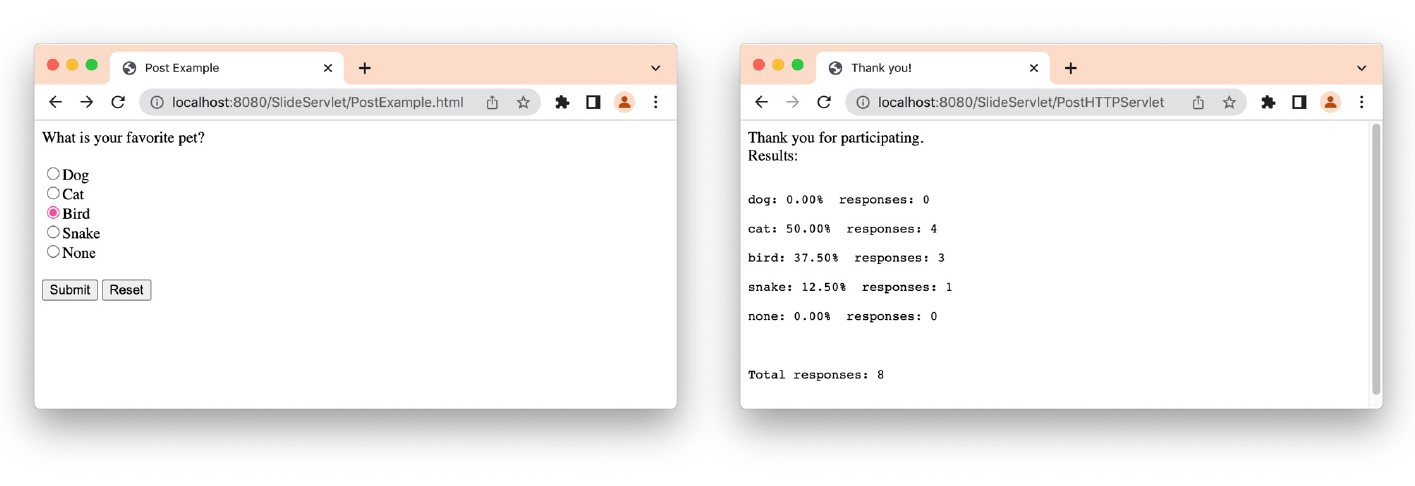
\includegraphics[width=0.5\textwidth]{img/appWeb8.jpg}
\end{center}

\subsubsection{Lato client: la pagina HTML}
\begin{verbatim}
    1. <html>
    2. <head>
    3. <meta charset="UTF-8">
    4. <title>Post Example</title>
    5. </head>
    6. <body>
    7.   <form action="http://localhost:8080/SlideServlet/PostHTTPServlet" method="POST">
    8.      What is your favorite pet?<br>
    9.      <br> <input type="radio" name="animal" value="dog">Dog<br>
    10.     <input type="radio" name="animal" value="cat">Cat<br> <input
    11.         type="radio" name="animal" value="bird">Bird<br> <input
    12.         type="radio" name="animal" value="snake">Snake<br> <input
    13.         type="radio" name="animal" value="none" checked>None <br><br>
    14.     <input type="submit" value="Submit"> <input type="reset">
    15.  </form>
    16.</body>
    17.</html>
\end{verbatim}

\subsubsection{Lato server: il metodo doPost}
\begin{verbatim}
    1. public class PostHTTPServlet extends HttpServlet {
    2.     // definisco l'elenco degli animali
    3.     private String animalNames[] = { "dog", "cat", "bird", "snake", "none" };
    4.     protected void doPost(HttpServletRequest request, HttpServletResponse response) {
    5.         int animals[] = null; // contatori di preferenze
    6.         int total = 0; // totale delle preferenze espresse
    7.         // i dati sono memorizzati nel file "survey.dat"
    8.         File f = new File("survey.dat"); // apro o creo il file
    9.         if (f.exists()) {
    10.             ObjectInputStream input = new ObjectInputStream(new FileInputStream(f));
    11.         try {
    12.             animals = (int[]) input.readObject(); // leggo il file e lo assegno a animals
    13.         } catch (ClassNotFoundException e) {
    14.             e.printStackTrace();
    15.         }
    16.         input.close(); // close stream
    17.         // conto quante sono le risposte date in precedenza
    18.         for (int i = 0; i < animals.length; ++i)
    19.             total += animals[i];
    20.         } else // creo un nuovo array di contatori
    21.             animals = new int[5];
    22.         // leggo il messaggio con la nuova preferenza
    23.         String value = request.getParameter("animal");
    24.         ++total; // aggiorno il totale delle risposte
    25.         // determino quello votato e aggiorno il suo contatore
    26.         for (int i = 0; i < animalNames.length; ++i)
    27.             if (value.equals(animalNames[i]))
    28.                 ++animals[i];
    29.         // scrivo i nuovi contatori sul file e lo chiudo
    30.         ObjectOutputStream output = new ObjectOutputStream(new FileOutputStream(f));
    31.         output.writeObject(animals);
    32.         output.flush();
    33.         output.close();
    34.         // calcolo le percentuali
    35.         double percentages[] = new double[animals.length];
    36.         for (int i = 0; i < percentages.length; ++i)
    37.             percentages[i] = 100.0 * animals[i] / total;
    38.         // uso un Buffer di servizio per costruire la pagina html in risposta
    39.         StringBuffer buf = new StringBuffer();
    40.         buf.append("<html>\n<title>Thank you!</title>\n");
    41.         buf.append("Thank you for participating.\n");
    42.         buf.append("<br>Results:\n<pre>");
    43.         DecimalFormat twoDigits = new DecimalFormat("#0.00");
    44.         for (int i = 0; i < percentages.length; ++i) {
    45.             buf.append("<br>" + animalNames[i] + ": " + twoDigits.format(percentages[i]));
    46.             buf.append("% responses: " + animals[i] + "\n");
    47.         }
    48.         buf.append("\n<br><br>Total responses: " + total);
    49.         buf.append("</pre>\n</html>");
    50.         // costruisco l'head del messaggio di risposta
    51.         response.setContentType("text/html"); // dichiaro il formato del body
    52.         // predispongo il canale stream per la scrittura del body del messaggio
    53.         PrintWriter responseOutput = response.getWriter();
    54.         // scrivo la pagina nella risposta
    55.         responseOutput.println(buf.toString());
    56.     }
    57. }
\end{verbatim}
Perché a 4. è protected? Perché deve essere ereditabile.

\subsection{Ciclo di vita di una servlet}
Una servlet viene creata dal container/engine:
\begin{itemize}
    \item Quando viene effettuata la prima chiamata
    \item La servlet viene condivisa da tutti client
    \item Ogni richiesta genera un \verb#Thread# che esegue la \verb#doXXX# appropriata
\end{itemize}
Il container/engine invoca il metodo \verb#init()# per inizializzazioni specifiche.
\\Una servlet viene distrutta dall'engine all'occorrenza di uno dei due eventi:
\begin{itemize}
    \item Quando non ci sono thread in esecuzione su quella servlet
    \item Quando è scaduto un timeout predefinito
\end{itemize}
Viene invocato il metodo \verb#destroy()# per terminare correttamente la servlet.
\begin{center}
    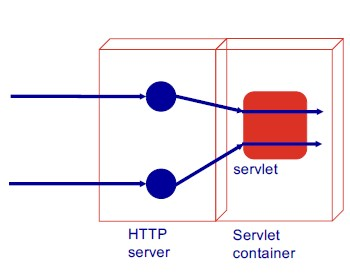
\includegraphics[width=0.5\textwidth]{img/appWeb9.jpg}
\end{center}
Una struttura del genere ha un nome, ma non ho capito quale. Penso "multitenant" perché ci sono più Client, ma ha senso come cosa?

\subsection{Servlet e Thread}
\begin{center}
    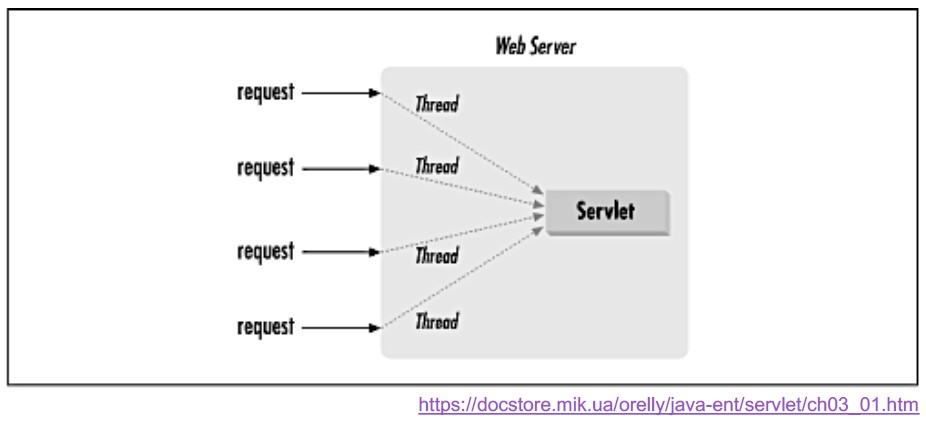
\includegraphics[width=0.5\textwidth]{img/appWeb10.jpg}
\end{center}
\begin{itemize}
    \item Molti thread -> una singola istanza della servlet
    \item Più richieste vengono servite dalla stessa servlet, questo vuol dire che bisogna far attenzione a come la servlet implementa l'accesso alle sue risorse
    \item In questo modello spesso le risorse sono condivise a livello di database
\end{itemize}
Questa scelta ha diverse motivazioni:
\begin{itemize}
    \item \underline{Utilizzare meno memoria} (un solo oggetto)
    \item \underline{Ridurre il costo di gestione} (per esempio tempi di inizializzazione inizializzazione) di molti oggetti che sarebbero spesso identici
    \item Abilita la persistenza (in memoria) di risorse condivisibili tra diverse richieste (e.g. una connessione a DB, oggetto "carrello")
\end{itemize}
Tornando all'esempio di prima, possiamo notare un problema abbastanza subdolo: non è gestito l'accesso in contemporanea al file. 
% Co-Pilot dice:
% Se due client inviano la loro preferenza nello stesso istante, il file potrebbe essere letto e scritto contemporaneamente, con conseguenze imprevedibili. Per risolvere questo problema, è necessario rendere la servlet thread-safe. Questo significa che la servlet deve essere in grado di gestire più richieste contemporaneamente, senza che si verifichino problemi di accesso alle risorse condivise. Per fare ciò, è necessario sincronizzare l'accesso alle risorse condivise. In questo caso, il file "survey.dat" è una risorsa condivisa, e quindi è necessario sincronizzare l'accesso a questo file. Per farlo, è sufficiente aggiungere la parola chiave synchronized davanti al metodo doPost. Il risultato è il seguente:

\subsection{Terminazione}
Container e richieste dei client devono sincronizzarsi sulla terminazione
\begin{itemize}
    \item Alla scadenza del \textit{timeout} potrebbe essere ancora dei thread in esecuzione in \verb#service()#
\end{itemize}
Bisogna:
\begin{itemize}
    \item Tener traccia dei \textit{thread} in esecuzione
    \item Progettare il metodo \verb#destroy()# in modo da notificare lo shutdown e attendere il completamento del metodo \verb#service()#
    \item Progettare i metodi lunghi in modo che verifichino periodicamente se è in corso uno shutdown e comportarsi di conseguenza
\end{itemize}

\subsection{Realizzazione di applicazioni}
Servlets "classiche", uso dell'ereditarietà. Supporta tutti i metodi.
\begin{center}
    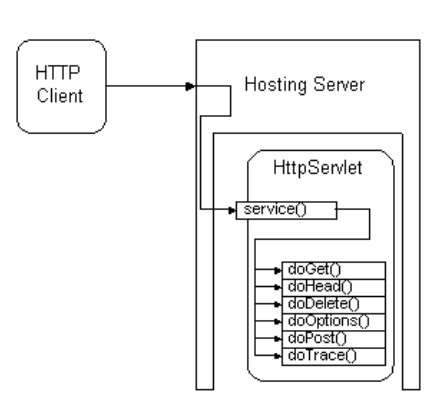
\includegraphics[width=0.5\textwidth]{img/appWeb11.jpg}
\end{center}
Spring MVC:
\begin{itemize}
    \item Spring@MVC, dalla versione 2.5 gestisce tutti i metodi HTTP
    \item Usa delle annotazioni per assegnare i metodi
\end{itemize}
\begin{center}
    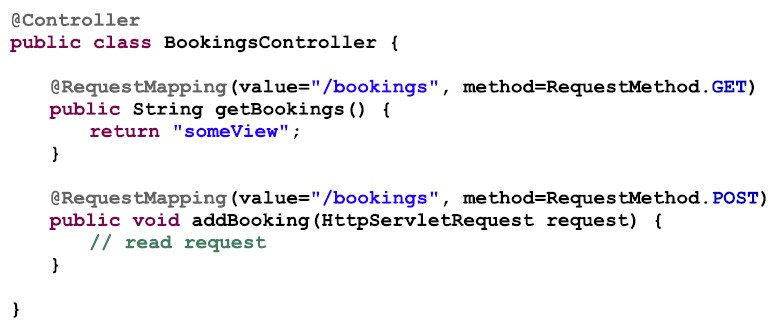
\includegraphics[width=0.675\textwidth]{img/appWeb12.jpg}
\end{center}
"@Controller" è un'annotazione di Java (e Spring) che indica che la classe è un controller. Vengono usate per arricchire la classe descrivendo cosa fa. In questo caso, la classe è un controller che gestisce le richieste HTTP.
\begin{center}
    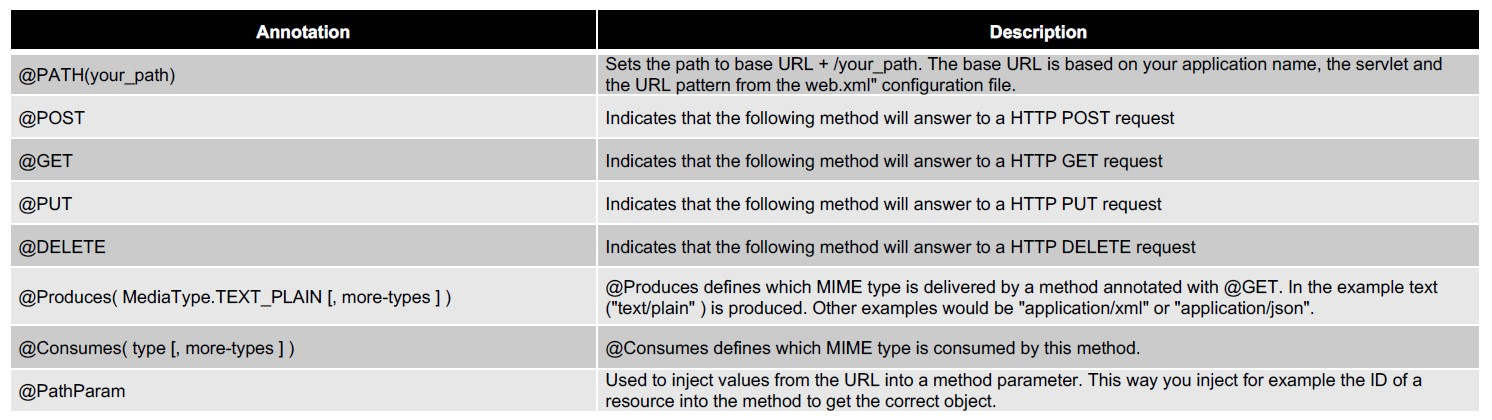
\includegraphics[width=0.5\textwidth]{img/appWeb13.jpg}
\end{center}
JAX-RS (e.g., jersey framework)
\begin{itemize}
    \item JSR 311
    \item Framework REST basato su annotazioni
\end{itemize}
\begin{center}
    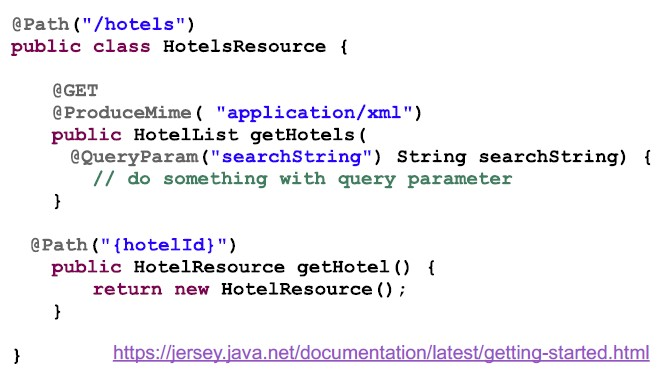
\includegraphics[width=0.5\textwidth]{img/appWeb14.jpg}
\end{center}

\section{SERVER SIDE - JSP}
JSP sta per Java Server Pages.

\subsection{Java Server Pages}
\`E una tecnologia per la creazione di applicazioni web. Specifica l'interazione tra un contenitore/server ed un insieme di "pagine" che presentano informazioni all'utente.
\\Le pagine sono costituite da tag tradizionali (HTML, XML, WML, …) e da tag applicativi che controllano la generazione del contenuto (generazione server-side).
\\JSP facilita la separazione tra logica applicativa e presentazione.
\\Analogo alla tecnologia Microsoft Active Server Page (ASP).
\\Differenze:
\begin{itemize}
    \item una Java Server Page chiama un programma Java eseguito sul Web server
    \item una Active Server Page contiene uno script VBScript o JScript
\end{itemize}
JavaServer Pages (JSP) separano la parte dinamica delle pagine dal template HTML statico.
\\Il codice JSP va incluso in tag delimitati da \begin{verbatim} "<%" e "%>".\end{verbatim}
Esempio
\begin{itemize}
    \item una pagina che visualizza
    \begin{verbatim}
        Grazie per la scelta di Internet Guida Pratica
    \end{verbatim}
    \item quando l'utente si connette all'URL
http://host/OrderConfirmation.jsp?title=Internet+Guida+Pratica
§ La JSP contiene
Grazie per la scelta di <i> <%= request.getParameter("title") %> </i>
§ La pagina viene convertita automaticamente in una servlet java la prima volta che viene richiesta.
Output:
\begin{center}
    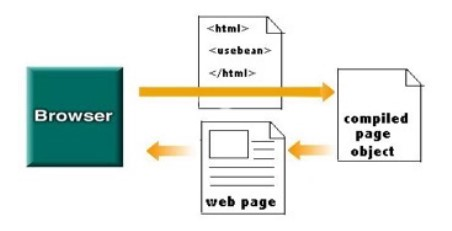
\includegraphics[width=0.675\textwidth]{img/appWeb15.jpg}
\end{center}

\subsection{Ciclo di vita delle applicazioni JSP}
\begin{center}
    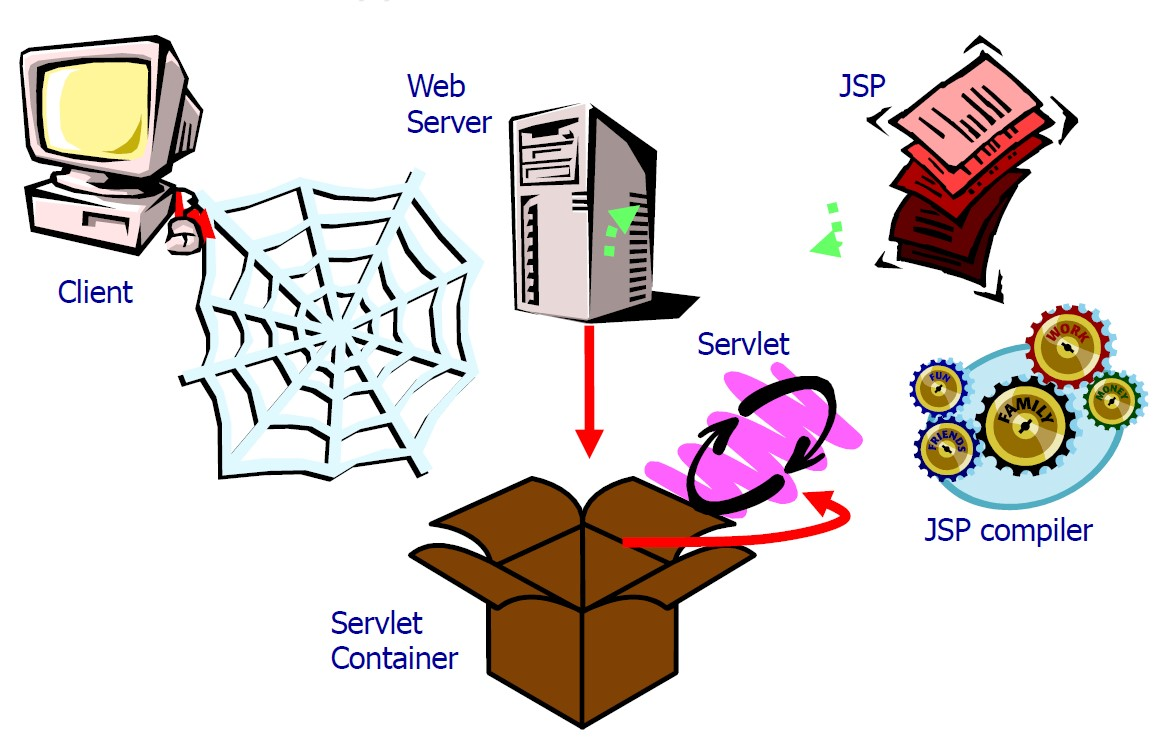
\includegraphics[width=0.5\textwidth]{img/appWeb16.jpg}
\end{center}

\subsection{JSP: esempio}
\begin{verbatim}
    1. <%@ page language="java" contentType="text/html; charset=UTF-8” pageEncoding="UTF-8"%>
    2. <!DOCTYPE html PUBLIC "-//W3C//DTD HTML 4.01 Transitional//EN" "http://www.w3.org/TR/html4/loose.dtd">
    3. <html>
    4. <head>
    5. <meta http-equiv="Content-Type" content="text/html; charset=UTF-8">
    6. <title>Welcome</title>
    7. </head>
    8. <body>
    9.     <h1> <%= "Welcome to JSP!" %> <h1>
    10. </body>
    11. </html>
\end{verbatim}

\subsection{Gli elementi di una JSP}
Template text
§ Le parti statiche della pagina HTML
§ Commenti
<%-- questo è un commento -->
§ Direttive
<%@ direttiva ... di compilazione %>
§ Azioni
<jsp:XXX attributes> body </jsp:XXX>
§ Elementi di scripting
§ Istruzioni nel linguaggio specificato nelle direttive
§ Sono di tre tipi: scriplet, declaration, expression

\subsubsection{Direttive}
Le direttive non influenzano la gestione di una singola richiesta
HTTP ma influenzano le proprietà generali della JSP e come questa
deve essere tradotta in una servlet.
page
§ Liste di attributi/valore
§ Valgono per la pagina in cui sono inseriti
<%@ page import="java.util.*" buffer="16k" %>
<%@ page import="java.math.*, java.util.*" %>
<%@ page session="false" %>
§ include
§ Include in compilazione pagine HTML o JSP
<%@ include file="copyright.html" %>
§ taglib
§ Dichiara tag definiti dall'utente implementando opportune classi
<%@ taglib uri="TableTagLibrary" prefix="table" %>
<table:loop> ... </table:loop>

\subsubsection{Azioni}
Le azioni permettono di supportare diversi comportamenti della pagina JSP.
Vengono processati ad ogni invocazione della pagina JSP. Permettono di trasferire
il controllo da una JSP all'altra, di interagire con i Java Data Beans, ecc.
forward
§ determina l'invio della richiesta corrente, eventualmente
aggiornata con ulteriori parametri, alla JSP indicata
<jsp:forward page="login.jsp" >
<jsp:param name="username" value="user" />
<jsp:param name="password" value="pass" />
</jsp:forward>
§ include
§ invia dinamicamente la richiesta ad una data URL e ne include il risultato
<jsp:include page="shoppingCart.jsp" />
§ useBean
§ localizza ed istanzia (se necessario) un javaBean nel contesto specificato
§ Il contesto può essere
§ La pagina, la richiesta, la sessione, l'applicazione
<jsp:useBean id="cart" scope="session" class="ShoppingCart" />
\begin{center}
    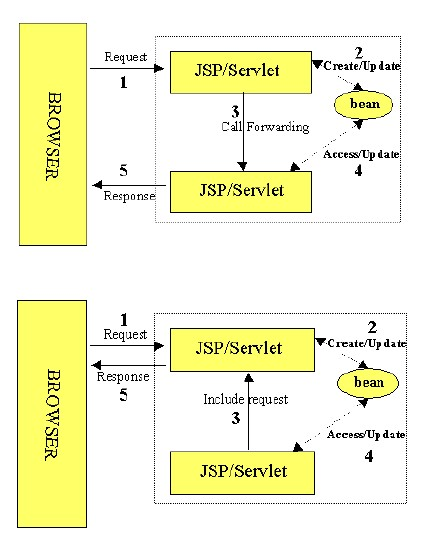
\includegraphics[width=0.5\textwidth]{img/appWeb18.jpg}
\end{center}

\subsubsection{Elementi di scripting}
Declaration <%! declaration [declaration] ... %>
§ Variabili o metodi statici usati nella pagina
<%! int[] v= new int[10]; %>
§ Expression <%= expression %>
§ Una espressione nel linguaggio di scripting (Java) che viene valutata e sostituita al tag
<p> La radice di 2 vale <%= Math.sqrt(2.0) %> </p>
§ Scriptlet <% codice %>
§ Frammenti di codice che controllano la generazione del codice HTML, valutati alla richiesta
§ Tale codice diventerà parte dei metodi doGet (doPost) della servlet che viene associata la JSP.
<table>
<% for (int i=0; i< v.length; i++) { %>
<tr><td> <%= v[i] %> </td></tr>
<% } %>
</table>
In questo modo riusciamo a superare un ostacolo importante di HTML che è la staticità.
\\Un linguaggio di script ha lo scopo di:
§ interagire con oggetti java e altre servlet
§ gestire le eccezioni java
§ Può utilizzare anche oggetti impliciti (sono 9)
§ request
§ response
§ out
§ page
§ pageContext
§ session
§ application
§ config
§ exception
Esempio:
Grazie per la scelta di <i> <%= request.getParameter("title") %> </i>

\subsection{Oggetti e loro "scope"}
Lo scope è la durata del ciclo di vita di un oggetto.
\\Gli oggetti possono essere creati
§ implicitamente usando le direttive JSP
§ esplicitamente con le azioni
§ direttamente usando uno script (raro)
§ Gli oggetti hanno un attributo che ne definisce lo “scope”
\begin{center}
    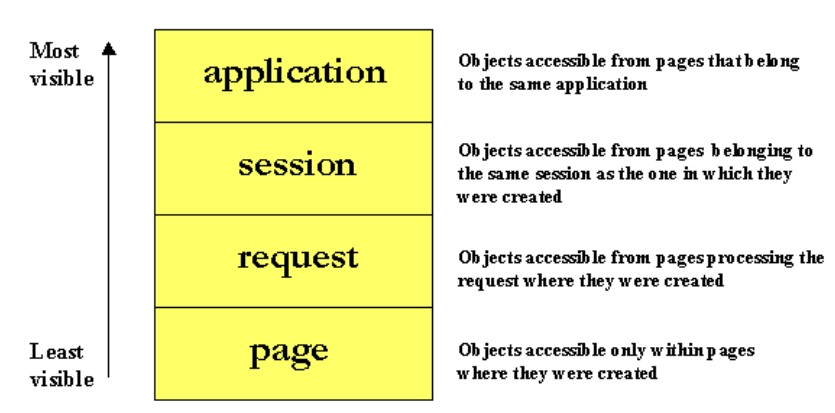
\includegraphics[width=0.5\textwidth]{img/appWeb19.jpg}
\end{center}

\subsection{JavaBeans}
Un javabean è una classe che segue regole precise (specifica)
§ Deve avere costruttori senza parametri
§ Dovrebbe avere campi (property) private
§ I metodi di accesso ai campi (property) sono set/get
setXxx
getXxx/isXxx
con xxx = property
\begin{verbatim}
    1. class Book{
    2.   private String title;
    3.   private boolean available;
    4.   void setTitle(String t) ...;
    5.   String getTitle() ...;
    6.   void setAvailable(boolean b) ...;
    7.   boolean isAvailable () ...;
    8. }
\end{verbatim}

\subsubsection{Azioni per utilizzare un bean}
Accedere ad un bean (inizializzazione)
\begin{verbatim}
    <jsp:useBean id="user" class="com.jguru.Person" scope="session" />
    <jsp:useBean id="user" class="com.jguru.Person" scope="session" >
        <% user.setDate(DateFormat.getDateInstance( ).format(new Date())); //etc.. %>
    </jsp:useBean>
\end{verbatim}
Accedere alle proprietà
\begin{verbatim}
    <jsp:getProperty name="user" property="name" />
    <jsp:setProperty name="user" property="name" value="jGuru" />
    <jsp:setProperty name="user" property="name" value="<%= expression %>" />
\end{verbatim}

\subsubsection{Accesso ad un JavaBean}
\begin{verbatim}
    <jsp:useBean id="Attore" class="MyThread" scope="session" type="Thread"/>
\end{verbatim}
Lo scope determina la vita e visibilità del bean:
\begin{description}
    \item[page:] è lo scope di default, viene messo in pageContext ed acceduto con getAttribute
    \item[request:] viene messo in ServletRequest ed acceduto con getAttribute
    \item[session e application:] se non esiste un bean con lo stesso id, ne viene creato uno nuovo
\end{description}
Il type permette di assegnargli una superclasse o un'interfaccia.
\\Al posto della classe si può usare il nome del bean
\begin{description}
    \item[beanName="nome"] nome è la classe o un file serializzato
\end{description}

\subsubsection{CounterBean.java}
\begin{verbatim}
    1. public class CounterBean {
        2. //declare a integer for the counter
        3. private int count;

        1. public int getCount() {
            2. //return count
            3. return count;
        4. }

        1. public void increaseCount() {
            2. //increment count
            3. count++;
        4. }
    5. }
\end{verbatim}

\subsubsection{Counter.java}
\begin{verbatim}
    1. <%@ page import="itis.mvc.CounterBean"%>
    2. <jsp:useBean id="session_counter" class="itis.mvc.CounterBean" scope="session" />
    3. <jsp:useBean id="app_counter" class="itis.mvc.CounterBean" scope="application" />
    4. <%
    5.   session_counter.increaseCount();
    6.   synchronized (page) {
    7.   app_counter.increaseCount();
    8. }
    9. %>
    10. <h3>
    11.     Number of accesses within this session:
    12.     <jsp:getProperty name="session_counter" property="count" />
    13. </h3>
    14. <p></p>
    15. <h3>
    16.     Total number of accesses:
    17.     <% synchronized (page) { %>
    18.     <jsp:getProperty name="app_counter" property="count" />
    19.     <% } %>
    20. </h3>
\end{verbatim}
\begin{center}
    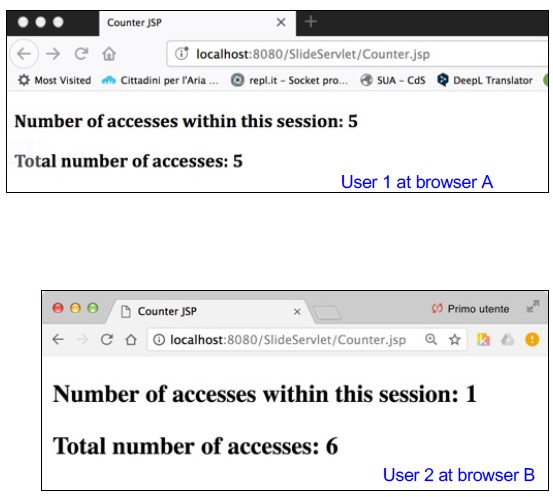
\includegraphics[width=0.675\textwidth]{img/appWeb20.jpg}
\end{center}

\subsection{Sessioni}
Accede ad un oggetto HTTPSession (session).
\\Mappa chiave-valore.
\begin{center}
    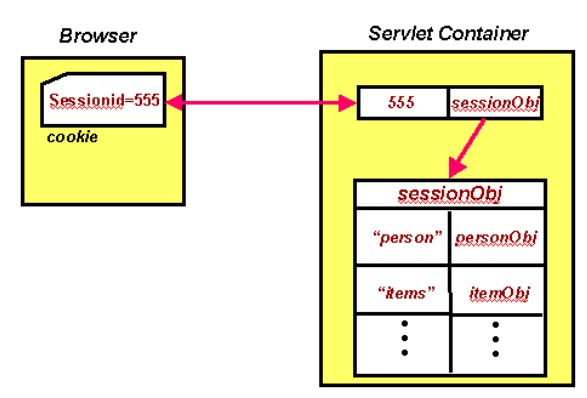
\includegraphics[width=0.675\textwidth]{img/appWeb21.jpg}
\end{center}
Esempi
\begin{itemize}
    \item Memorizzazione
    \begin{verbatim}
        <% Foo foo = new Foo(); session.putValue("foo",foo); %>
    \end{verbatim}
    \item Recupero
    \begin{verbatim}
        <% Foo myFoo = (Foo) session.getValue("foo"); %>
    \end{verbatim}
    \item Esclusione di una pagina dalla sessione
    \begin{verbatim}
        <%@ page session="false" %>
    \end{verbatim}
\end{itemize}

\subsection{Altro esempio: uso di dati dinamici}
\begin{verbatim}
    1. <%@ page language="java" contentType="text/html; charset=UTF-8" pageEncoding="UTF-8"%>
    2. <!DOCTYPE html PUBLIC "-//W3C//DTD HTML 4.01 Transitional//EN" "http://www.w3.org/TR/html4/loose.dtd">
    3. <html>
    4. <head>
    5. <meta http-equiv="Content-Type" content="text/html; charset=UTF-8">
    6. <title>Uso di JSP</title>
    7. <link rel=”stylesheet" href="My-Style-Sheet.css" type="text/css”>
    8. </head>
    9. <body bgcolor="#FDF5E6" text="blue">
    10.     <center>
    11.         <table border="5" bgcolor="#EF8429">
    12.             <tr>
    13.                 <th class="title"> Using JavaServer Pages </th>
    14.             </tr>
    15.         </table>
    16.     </center>
    17.     <br> Some dynamic content created using various JSP mechanisms:
    18.     <ul>
    19.         <li><b>Expression.</b><br> Your hostname: <%=request.getRemoteHost()%>. </li>
    20.         <li><b>Scriptlet.</b><br> <% out.println("Attached GET data: " + request.getQueryString()); %></li>
    21.         <li><b>Declaration (plus expression).</b><br> <%!private int accessCount = 0;%>
    22.             Accesses to page since server reboot: <%=++accessCount%> </li>
    23.         <li><b>Directive (plus expression).</b><br> <%@ page import="java.util.*"%> Current date: <%=new Date()%> </li>
    24.     </ul>
    25. </body>
    26. </html>
\end{verbatim}
Output:
\begin{center}
    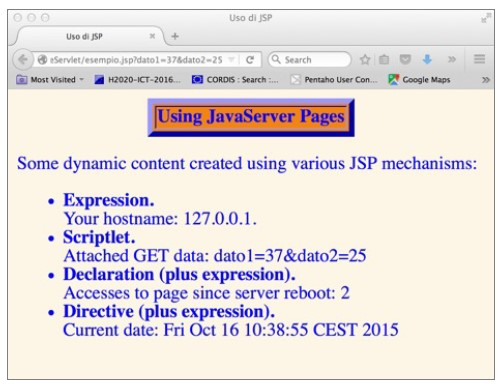
\includegraphics[width=0.675\textwidth]{img/appWeb22.jpg}
\end{center}

\subsection{Es. JSP con Form HTML}
\begin{verbatim}
1. <!DOCTYPE html>
2. <html>
3. <head>
4. <meta charset="UTF-8">
5. <title>JSP Example</title>
6. </head>
7. <body>

8. <form action="http://localhost:8080/SlideServlet/FC.jsp" method="GET">
9.      Converter <br><br>
10.     <input type="radio" name="unit" value="celsius">Celsius<br>
11.     <input type="radio" name="unit" value="fahrenheit">Fahrenheit<br>
12.     value <input type="text" name="value" ><br><br>
13.     <input type="submit" value="send">
14.     <input type="reset">
15.</form>

16.</body>
17.</html>
\end{verbatim}

\subsubsection{FC converter in versione JSP}
\begin{verbatim}
    1. <%@ page language="java" contentType="text/html; charset=UTF-8" pageEncoding="UTF-8"%>
    2. <!DOCTYPE html PUBLIC "-//W3C//DTD HTML 4.01 Transitional//EN" "http://www.w3.org/TR/html4/loose.dtd">
    3. <html><head><meta http-equiv="Content-Type" content="text/html; charset=UTF-8">
    4. <title>F2C converter</title></head>
    5. <body>
    6. <%@ page import = "java.text.DecimalFormat" %>
    7. <% Double result;
    8. String unit = request.getParameter("unit");
    9. Double value=Double.parseDouble(request.getParameter("value")); %>
    10. <h1> <% if( unit.equals("fahrenheit")) { %>
    11. Fahrenheit to Celsius
    12. <% result=(value - 32) * 5 / 9;
    13. } else { %>
    14. Celsius to Fahrenheit
    15. <% result=((value * 9) / 5) + 32; } %>
    16. </h1>
    17. <% DecimalFormat twoDigits = new DecimalFormat( "#0.00" ); %>
    18. <h2> <%= unit %> : <%= twoDigits.format(value) %> </h2>
    19. <h2> <% if( unit.equals("fahrenheit")) { %>
    20. fahrenheit:
    21. <%
    22. } else { %>
    23. celsius:
    24. <% } %>
    25. <%= twoDigits.format( result ) %>
    26. </h2>
    27. </body>
    28. </html>
\end{verbatim}

\section{Il pattern MVC - Model View Control}
\subsection{Il pattern MVC}
Il pattern Model View Controller (MVC) ha lo scopo di separare
\begin{itemize}
    \item I dati e i metodi principali per la loro manipolazione (Model)
    \item La presentazione, cioè l'interfaccia (View)
    \item Il coordinamento dell'interazione tra interfaccia (azioni degli utenti) e i dati (Controller)
\end{itemize}
\begin{center}
    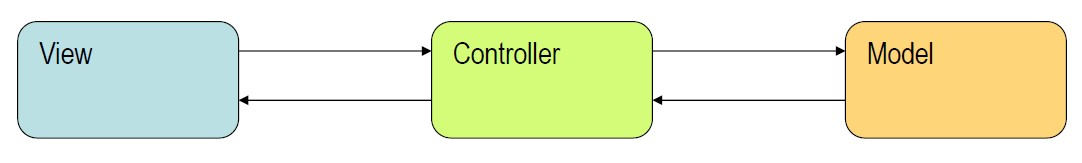
\includegraphics[width=0.675\textwidth]{img/appWeb24.jpg}
\end{center}

\subsection{Il design pattern MVC}
Il Model-View-Controller (MVC) è un pattern architetturale che separa data model, user interface, e control logic in tre
componenti distinte
§ Model
§ I dati (gli oggetti) trattati dall'applicazione, e le operazioni su di essi
§ View
§ La struttura dei dati restituiti al richiedente (e.g., la pagina HTML/CSS)
§ Control
§ Definisce le azioni da eseguire a fronte di una richiesta
§ Interagisce con il Model per modificare i dati e con la View per generare la risposta
\begin{center}
    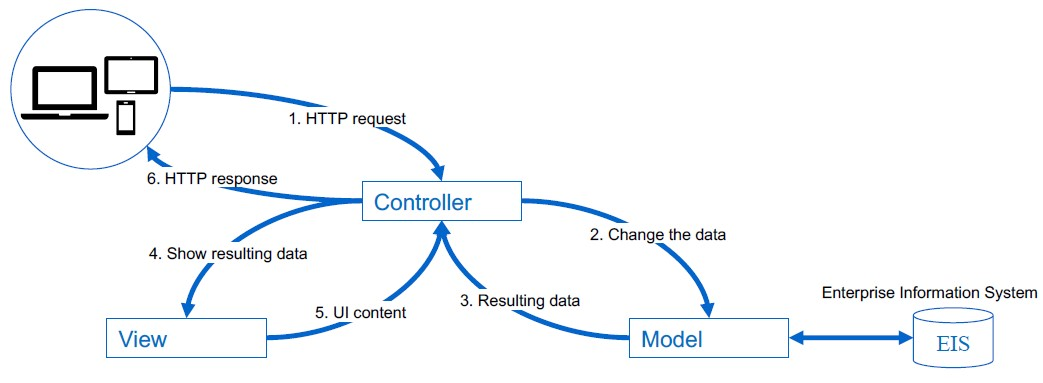
\includegraphics[width=0.5\textwidth]{img/appWeb25.jpg}
\end{center}
\begin{center}
    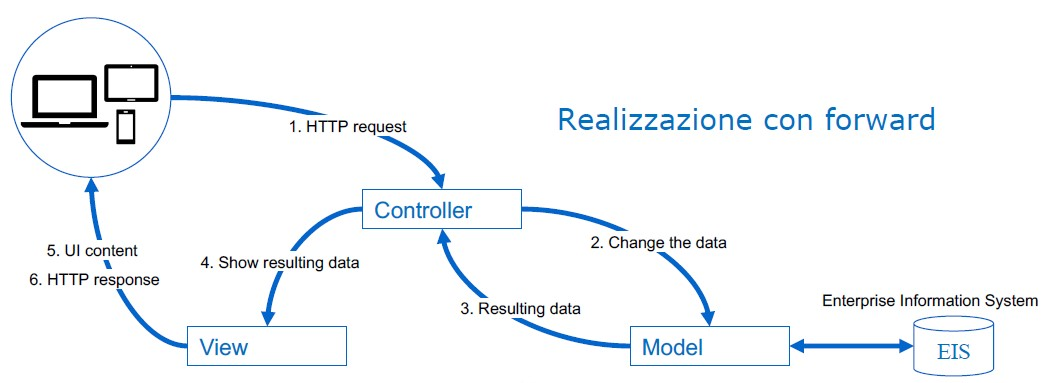
\includegraphics[width=0.5\textwidth]{img/appWeb26.jpg}
\end{center}

\subsection{Vantaggi e svantaggi}
\subsubsection{Vantaggi:}
Chiara separazione tra logica di business e logica di presentazione
§ poter cambiare la view senza modificare il control e viceversa
§ poter arricchire la view senza appesantire il codice del controller
§ poter definire e scegliere a run-time la view da usare a seconda dell'interazione, dei device utilizzati, dello stato dei dati o delle
preferenze dell'utente
§ Chiara separazione tra logica di business e modello dei dati
§ poter definire diversi mapping tra le azioni degli utenti sul controller e le funzioni sul model
§ Ogni componente ha una responsabilità ben definita
§ poter sviluppare in parallelo
§ poter manutenere e far evolvere ogni componente in modo indipendente, quindi semplificando la gestione
§ Ogni parte può essere affidata a esperti
§ poter assegnare lo sviluppo della view ad esperti di interfaccia e interazione (e.g., pagine jsp o asp)
§ uso tecnologie adatte allo sviluppo delle singole componenti
\subsubsection{Svantaggi:}
Aumento della complessità dovuta alla concorrenza (è un sistema distribuito).
\\Inefficienza nel passaggio dei dati alla view (un elemento in più tra cliente e controller).

\subsection{Il pattern Model 1}
Scopo: separazione tra dati, logica di busines e visualizzazione
\begin{enumerate}
    \item Il browser invia una richiesta per la pagina JSP
    \item JSP accede a Java Bean e invoca la logica di business
    \item Java Bean si connette al database e ottiene/salva i dati
    \item La risposta, generata da JSP, viene inviata al browser
\end{enumerate}
Architettura tipica: